\documentclass[11pt]{article}
\usepackage[margin=1in]{geometry}
\usepackage{amsmath,amssymb,amsthm,mathtools,bm}
\usepackage{booktabs,array,tabularx,multirow}
\usepackage{graphicx}
\usepackage{xcolor}
\usepackage{microtype}
\usepackage{enumitem}
\usepackage{hyperref}
\usepackage[nameinlink,capitalise]{cleveref}
\usepackage{authblk}
\usepackage{caption}
\usepackage{subcaption}
\usepackage{float}
\usepackage{longtable}
\usepackage{siunitx}
\graphicspath{{qubit/results/figures/}{qutrit/figures/}}
\hypersetup{colorlinks=true,linkcolor=blue!55!black,citecolor=green!35!black,urlcolor=blue!55!black}
\setlist{nosep}
\newtheorem{theorem}{Theorem}[section]
\newtheorem{proposition}[theorem]{Proposition}
\newtheorem{lemma}[theorem]{Lemma}
\newtheorem{corollary}[theorem]{Corollary}
\theoremstyle{definition}
\newtheorem{definition}[theorem]{Definition}
\newtheorem{example}[theorem]{Example}
\newtheorem{criterion}[theorem]{Criterion}
\theoremstyle{remark}
\newtheorem{remark}[theorem]{Remark}
\newcommand{\cH}{\mathcal H}
\newcommand{\cA}{\mathcal A}
\newcommand{\cO}{\mathcal O}
\newcommand{\cE}{\mathcal E}
\newcommand{\cU}{\mathcal U}
\newcommand{\cS}{\mathcal S}
\newcommand{\cT}{\mathcal T}
\newcommand{\Tr}{\operatorname{Tr}}
\newcommand{\id}{\mathsf{id}}
\newcommand{\rank}{\operatorname{rank}}
\newcommand{\TV}{\operatorname{TV}}
\newcommand{\JS}{\operatorname{JS}}
\newcommand{\R}{\mathbb R}
\newcommand{\C}{\mathbb C}
\newcommand{\Z}{\mathbb Z}
\title{\textbf{Informative Quantum Actions and Predictive Goal Geometry}\\
\large Operational Meaning, Low-Dimensional Constructions, and an Exact Bellman Obstruction}
\author{Quantum Hodology Research Project}
\date{\today}
\begin{document}
\maketitle

\begin{abstract}
Can an agent learn that its available quantum interventions mean
\textquotedblleft move north,\textquotedblright\ \textquotedblleft move
east,\textquotedblright\ and so forth, without those meanings being supplied
as labels? This paper develops an operational framework in which an action is
defined by the future outcome statistics it induces. Controlled quantum
instruments generate histories; equivalence of histories under all future
tests defines predictive states; and equivalence of actions is quotienting by
every experimentally invisible realization gauge. Goal-directed control then
equips predictive states with Bellman costs. A two-dimensional hodological
space exists only when these costs pass metric and Euclidean embeddability
tests, most sharply Schoenberg's centered-Gram criterion.

Two low-dimensional studies make the distinction between \emph{information}
and \emph{geometry} concrete. A qubit instrument has an exactly invertible
predictive phase chart and its two opaque actions are learned from present and
future data, but its nonunitary dynamics fail path-independent composition. A
qutrit Hesse-SIC instrument is more strongly integrated: every action both
translates a hidden \(\Z_3^2\) label and reports a noisy outcome. From shuffled
tokens alone, maximum-likelihood transition tables recover the toroidal action
topology exactly. Nevertheless, its undiscounted Bellman goal cost is \(4\)
both at a goal and at an adjacent state, violating identity of
indiscernibles. Weakening the measurement does not repair this equality.
Separating motion from reporting gives the exact benchmark
\(V_g(s)=6+d_T(s,g)\), but no longer solves the integrated-action problem.

The resulting lesson is constructive but deliberately limited. Small Hilbert
spaces can support learned operational action semantics and exact finite
topology. They do not automatically produce a metric merely because their
latent action graph is spatial. We prove a no-information-without-disturbance
theorem under explicit universal assumptions, state finite
necessary-and-sufficient criteria for predictive two-dimensional geometry,
and propose a program based on weak covariant instruments, predictive atlases,
and control-aware measurement design.
\end{abstract}
\tableofcontents

\section{Why action meaning should be operational}

The motivating hypothesis is that space need not be a primitive arena. For a
goal-directed agent, a goal reached cheaply is near and one requiring many
risky or costly interventions is far. A geometry reconstructed from such
costs is \emph{hodological}: it is a geometry of routes, obstacles, and
attainability. If a family of goals admits a faithful two- or
three-dimensional embedding, an agent's policy may be interpreted as motion
through an emergent space.

There is an important circularity to avoid. If the experimenter names two
buttons \(X\) and \(Y\), declares that they translate horizontal and vertical
coordinates, and scores the agent by distance on that declared grid, the
spatial interpretation was inserted before learning. The stronger question is:
\begin{quote}
Can the agent infer the operational meanings of opaque interventions from
outcome statistics, then discover that its goal costs possess low-dimensional
spatial structure?
\end{quote}
The phrase \emph{operational meaning} is essential. Quantum channels have many
equivalent Kraus and coordinate descriptions. Only probabilities of possible
future experiments can be learned. We therefore build the theory from
histories and tests, not from a preferred matrix representation.

This paper separates four questions that are often conflated:
\begin{enumerate}
\item \textbf{Immediate informativeness:} does the outcome emitted by the
current action depend on the current predictive state?
\item \textbf{Future-operational action meaning:} can two actions be
distinguished by some later controlled experiment, even if their immediate
outcome laws coincide?
\item \textbf{Compositional topology:} do learned action maps close into a
stable graph or group-like structure?
\item \textbf{Hodological geometry:} do optimal goal costs define a genuine
metric, and is that metric Euclidean in low dimension?
\end{enumerate}
Our exact qutrit example answers the first three positively and the fourth
negatively. That separation is one of the central results.

\section{Controlled quantum experiments from first principles}

\subsection{States, channels, and instruments}

Let \(\cH\simeq\C^d\). A quantum state is a positive semidefinite operator
\(\rho\succeq0\) with \(\Tr\rho=1\). A quantum channel is a completely
positive, trace-preserving linear map. A \emph{controlled instrument} for
action \(a\in\cA\) is a finite set
\[
\mathfrak I^a=\{\cE^a_o:o\in\cO_a\}
\]
of completely positive, trace-nonincreasing maps whose sum
\(\Phi_a=\sum_o\cE^a_o\) is trace preserving
\cite{Kraus1983,NielsenChuang2010}. When
\(\cE^a_o(\rho)=K_{a,o}\rho K_{a,o}^\dagger\),
\(\sum_oK_{a,o}^\dagger K_{a,o}=I\). More general outcomes may have several
Kraus operators.

For state \(\rho\), the probability and normalized posterior are
\[
p(o\mid \rho,a)=\Tr[\cE^a_o(\rho)],\qquad
\rho'=\frac{\cE^a_o(\rho)}{p(o\mid\rho,a)}.
\]
The outcome-forgotten state is \(\Phi_a(\rho)\). This distinction between
selective and nonselective evolution matters throughout.

\subsection{Histories, tests, and the system-dynamics matrix}

A history is an observed string
\[
h=(a_1,o_1)\cdots(a_t,o_t).
\]
Its unnormalized state is
\[
\widetilde\rho_h=
\cE^{a_t}_{o_t}\circ\cdots\circ\cE^{a_1}_{o_1}(\rho_0),
\qquad p(h)=\Tr\widetilde\rho_h.
\]
A test \(\tau=(b_1,y_1)\cdots(b_k,y_k)\) specifies future controls and queried
outcomes. Conditional on a possible history,
\[
p(\tau\mid h)=
\frac{\Tr[\cE^{b_k}_{y_k}\circ\cdots\circ\cE^{b_1}_{y_1}
(\widetilde\rho_h)]}{\Tr\widetilde\rho_h}.
\]
Arrange these probabilities into the generally infinite Hankel or
system-dynamics matrix
\[
\mathbf H_{h,\tau}=p(\tau\mid h).
\]
This contains precisely the controlled input--output behavior. A
predictive-state representation (PSR) chooses core tests
\(\tau_1,\ldots,\tau_r\) and represents a history by
\[
q(h)=\bigl(p(\tau_1\mid h),\ldots,p(\tau_r\mid h)\bigr).
\]
When the Hankel rank is \(r<\infty\), all test predictions are linear
functionals of an \(r\)-dimensional predictive state \cite{Littman2001}.

\begin{definition}[Predictive or causal equivalence]
Histories \(h,h'\) satisfy \(h\sim h'\) when
\[
p(\tau\mid h)=p(\tau\mid h')
\quad\text{for every admissible future test }\tau.
\]
The quotient classes are the agent's operational states.
\end{definition}

This definition is stricter than equality under one measurement and weaker
than equality of density matrices. Restricted controls may leave distinct
density operators operationally indistinguishable. Conversely, a classical
memory state attached to the controller may distinguish histories even when
the physical density operator does not. Physical Hilbert dimension,
predictive dimension, and controller-memory dimension are therefore different
resources.

\begin{proposition}[Finite observability criterion]
For a finite candidate set \(S=\{s_1,\ldots,s_n\}\), the states are
operationally observable if and only if there exists a finite set of tests
\(T\) such that the row vectors
\(\bigl(p(\tau\mid s_i)\bigr)_{\tau\in T}\) are pairwise distinct.
\end{proposition}
\begin{proof}
If such a finite set exists, every pair is separated by one of its tests.
Conversely, if every pair is predictively inequivalent, choose one separating
test for each of the finitely many pairs and take their union.
\end{proof}

\subsection{Action equivalence and gauges}

An opaque action token has meaning only through how it transforms future
predictions. For a predictive state \(q\), define the outcome-labelled update
kernel
\[
T_a(q;o)=\bigl(p(o\mid q,a),q_{a,o}\bigr).
\]
Two actions are operationally equivalent if these kernels agree on all
reachable predictive states, or equivalently if their shifted Hankel blocks
\[
\mathbf H^{(a,o)}_{h,\tau}=p(o,\tau\mid h,a)
\]
agree for every \(o,h,\tau\).

Internal coordinates are not unique. A minimal linear PSR admits similarity
transformations \(q\mapsto Sq\), accompanied by inverse transformations of
test functionals. Gate-set tomography likewise has a similarity gauge that
leaves every circuit probability invariant \cite{NielsenGST2020,DiMatteo2020}.
State labels may be permuted, and a recovered square chart is ambiguous under
rotations and reflections. These are not estimation failures. A scientifically
meaningful reconstruction must be scored after quotienting by all such
operational gauges.

\begin{proposition}[Finite action-identifiability criterion]
Let \(S\) and \(\cA\) be finite and suppose \(S\) is observable. Distinct
action meanings are identifiable from controlled statistics if and only if,
for every \(a\ne b\), there exist \(s\in S\), an immediate outcome \(o\), and
a finite continuation test \(\tau\) such that
\[
p(o,\tau\mid s,a)\ne p(o,\tau\mid s,b).
\]
\end{proposition}
\begin{proof}
The displayed inequality is a finite experimental witness separating the two
shifted Hankel blocks, so it is sufficient. If no witness exists, every
admissible experiment has the same law after \(a\) and \(b\); no estimator can
distinguish them, so it is necessary.
\end{proof}

\section{Information, disturbance, and distinguishability}

\subsection{Several inequivalent notions of informativeness}

Let a random variable \(S\) index predictive states with prior \(\pi_s\). For
fixed action \(a\), immediate information is
\[
I(S;O\mid A=a)=
\sum_{s,o}\pi_s p(o\mid s,a)
\log_2\frac{p(o\mid s,a)}{\sum_{s'}\pi_{s'}p(o\mid s',a)}.
\]
It vanishes precisely when the current outcome law is state independent. But
\(I(S;O\mid A=a)=0\) does not imply that the action is meaningless: two
actions may prepare different posterior states that a later probe
distinguishes.

Local parametric sensitivity can be measured by classical Fisher information,
\[
F_a(\theta)=\sum_o p(o\mid\theta,a)
[\partial_\theta\log p(o\mid\theta,a)]^2.
\]
Global separation of two outcome laws can use total variation,
\(\TV(p,q)=\frac12\sum_o|p_o-q_o|\), or Jensen--Shannon divergence. At the
channel level, optimal distinguishability with arbitrary ancillas is governed
by the diamond norm \(\|\Phi_a-\Phi_b\|_\diamond\) \cite{Watrous2018}. These
quantities answer different questions and should not be collapsed into one
score.

Disturbance also requires an explicit reference task. For a pure input,
survival fidelity is
\[
F_{\rm surv}(\psi,a)=
\langle\psi|\Phi_a(|\psi\rangle\langle\psi|)|\psi\rangle.
\]
Trace distance, entanglement fidelity, or loss of future reward may be more
appropriate in other experiments. An information--disturbance plot is
meaningful only after both axes have been declared.

\subsection{Exact no information without universal nondisturbance}

\begin{theorem}[No information without disturbance under a unitary sum]
\label{thm:noinfo}
Let \(\{\cE_o\}\) be an instrument on a finite-dimensional system. Suppose its
nonselective channel equals a fixed unitary channel on the entire operator
space:
\[
\sum_o\cE_o=\cU,\qquad \cU(\rho)=U\rho U^\dagger.
\]
Then there are probabilities \(p_o\ge0\), \(\sum_op_o=1\), such that
\[
\cE_o=p_o\cU.
\]
Consequently \(p(o\mid\rho)=p_o\) is independent of the input state.
\end{theorem}
\begin{proof}
Let \(J(\Lambda)\) denote the Choi matrix of a completely positive map. Each
\(J_o=J(\cE_o)\) is positive semidefinite and
\[
\sum_oJ_o=J(\cU)=|U\rangle\!\rangle\langle\!\langle U|,
\]
which has rank one. If positive semidefinite matrices sum to a rank-one
matrix, every summand has support inside that same one-dimensional support.
Hence \(J_o=p_oJ(\cU)\) for some \(p_o\ge0\). The Choi isomorphism gives
\(\cE_o=p_o\cU\); trace preservation of the sum gives \(\sum_op_o=1\).
Finally \(\Tr\cE_o(\rho)=p_o\Tr\rho=p_o\).
\end{proof}

\begin{remark}[Why the assumptions matter]
The theorem asserts exact, universal preservation up to one unitary. A
quantum nondemolition measurement may reveal which member of an orthogonal or
commuting restricted family was supplied. A measurement may preserve an
average state without preserving each input. Syndrome extraction may disturb
a physical system while preserving an encoded logical subsystem. Approximate
preservation permits quantitative information--disturbance tradeoffs. None
contradicts \cref{thm:noinfo}.
\end{remark}

The theorem explains why an integrated spatial action faces tension. To
report where the agent is, an instrument must usually disturb some states. To
compose as a clean translation, it should preserve the degrees of freedom
that carry position except for the intended motion. The design problem is to
optimize this tension.

\section{From reinforcement learning to goal geometry}

\subsection{Policies, rewards, and Bellman equations}

Reinforcement learning studies sequential decisions. At time \(t\), an agent
has an operational state \(s_t\), chooses \(a_t\), observes an outcome and
incurs a cost. A policy \(\pi(a\mid s)\) specifies action probabilities. For a
discounted task,
\[
V^\pi(s)=\mathbb E_\pi\left[
\sum_{t=0}^\infty\gamma^t c(s_t,a_t,o_{t+1})
\middle|s_0=s\right],\qquad 0\le\gamma<1.
\]
The optimal value satisfies
\[
V(s)=\min_a\sum_o p(o\mid s,a)
\left[c(s,a,o)+\gamma V(f(s,a,o))\right].
\]
For stochastic-shortest-path problems one commonly sets \(\gamma=1\), unit
cost per intervention, and terminates upon verified goal success. Properness
conditions are then needed to ensure finite values and select the minimal
nonnegative Bellman solution \cite{Puterman1994,SuttonBarto2018}.

For goal \(g\), let \(V_g(s)\) be the optimal expected cost to attain and
verify \(g\). A raw directed hodological dissimilarity is
\[
C(s,g)=V_g(s)-V_g(g).
\]
Subtracting the self-cost is important when verification is noisy and costly.
One may symmetrize by
\[
D_{sg}=\tfrac12[C(s,g)+C(g,s)],
\]
but symmetrization alone does not enforce positivity or the triangle
inequality.

\subsection{Metric and Euclidean tests}

A distance matrix \(D\) is a metric when it is symmetric, nonnegative, zero
only on the diagonal, and obeys \(D_{ij}\le D_{ik}+D_{kj}\). To ask whether it
is exactly Euclidean, let \(J=I-\frac1n\mathbf1\mathbf1^T\) and form
\[
B=-\frac12J(D^{\circ2})J.
\]

\begin{theorem}[Schoenberg criterion]
\label{thm:schoenberg}
A finite symmetric matrix \(D\) with zero diagonal is realizable as Euclidean
distances among points in \(\R^k\) if and only if \(B\succeq0\) and
\(\rank B\le k\) \cite{Schoenberg1935}.
\end{theorem}
\begin{proof}
If \(D_{ij}=\|x_i-x_j\|_2\) and the coordinates are centered, expanding
squared distances gives \(B=XX^T\succeq0\), with rank at most \(k\).
Conversely, diagonalize \(B=Q\Lambda Q^T\). When \(B\succeq0\), take
\(X=Q\Lambda^{1/2}\) using its positive eigenvalues. Double centering
guarantees that pairwise squared distances between rows of \(X\) equal
\(D_{ij}^2\). The number of positive eigenvalues is the embedding dimension.
\end{proof}

When exact embeddability fails, classical multidimensional scaling retains the
leading positive eigenvalues. Stress summarizes distortion, but a visually
pleasing plot is not a proof. In particular, a finite torus has a legitimate
two-generator topology while its all-pairs word metric need not embed
isometrically in the Euclidean plane.

\subsection{Finite necessary-and-sufficient certificate}

\begin{criterion}[Predictive two-dimensional hodology]
\label{crit:atlas}
For finite histories, tests, actions, and goals, a statistics-learnable exact
two-dimensional hodological geometry exists if and only if all of the
following hold on the operational quotient:
\begin{description}
\item[(P)] chosen predictive states have distinct finite Hankel rows;
\item[(A)] intended action meanings have distinct finite shifted-Hankel blocks;
\item[(B)] every goal Bellman equation has a finite minimal nonnegative
solution under the declared costs and stopping rule;
\item[(M)] the resulting \(D\) is a metric;
\item[(E)] \(B=-\frac12JD^{\circ2}J\succeq0\) and \(\rank B\le2\).
\end{description}
If actions are additionally to mean homogeneous local translations, require:
\begin{description}
\item[(L)] recovered action kernels are local in the embedding and their
coordinate displacement laws are state independent up to admitted boundary
or gauge symmetries.
\end{description}
\end{criterion}

\begin{proof}
Necessity follows directly: learned states and actions must be statistically
separable; values must exist; Euclidean distance is a metric and satisfies
\cref{thm:schoenberg}; homogeneous translations have the stated covariance.
For sufficiency, (P) and (A) identify the finite operational model from
statistics up to gauge. Solve the Bellman systems by (B), construct \(D\) by
(M), and use the eigenfactorization in \cref{thm:schoenberg} to obtain
coordinates in \(\R^2\). Condition (L) then assigns learned displacement
semantics to actions. Coordinates are unique only up to Euclidean isometry
when the distance data are complete and span the plane.
\end{proof}

This criterion is intentionally modular. The qutrit experiment below passes
(P), (A), and a topological analogue of (L), but fails (M). That is a sharper
diagnosis than reporting a single embedding stress.

\section{Qubit case study: an exact predictive action chart}
\label{sec:qubit}

\subsection{Instrument and exact probability laws}

The first construction asks how much operational semantics a single qubit can
carry. Reset the qubit to
\[
\rho_0=|{+x}\rangle\langle{+x}|=\tfrac12(I+X).
\]
An opaque action \(b\) applies a \(Z\)-rotation
\[
U_{\theta_b}=e^{-i\theta_b Z/2}
\]
and then an unsharp binary \(X\)-measurement with effects
\[
E_o=\tfrac12(I+osX),\qquad o\in\{+1,-1\},\quad 0<s<1.
\]
A Lüders realization is
\[
K_{b,o}=\sqrt{E_o}\,U_{\theta_b},\qquad
\cE^b_o(\rho)=K_{b,o}\rho K_{b,o}^\dagger.
\]
Completeness follows from \(\sum_oE_o=I\). After the rotation, the reset Bloch
vector is \((\cos\theta_b,\sin\theta_b,0)\), so the immediate outcome law is
\begin{equation}
\label{eq:qubit-immediate}
p(+\mid b)=\Tr(E_+U_{\theta_b}\rho_0U_{\theta_b}^\dagger)
=\frac{1+s\cos\theta_b}{2}.
\end{equation}
Thus the current outcome learns only the cosine of the phase. It cannot
distinguish \(\theta\) from \(-\theta\).

The nonselective Lüders measurement dephases perpendicular to the \(X\)-axis.
Writing
\[
\eta=\sqrt{1-s^2},
\]
the outcome-forgotten post-action Bloch vector is
\[
r_b=(\cos\theta_b,\eta\sin\theta_b,0).
\]
Two future probes close the chart:
\begin{equation}
\label{eq:qubit-probes}
p(X+\mid b)=\frac{1+\cos\theta_b}{2},\qquad
p(Y+\mid b)=\frac{1+\eta\sin\theta_b}{2}.
\end{equation}
Therefore, for known \(s<1\),
\begin{equation}
\label{eq:phase-recovery}
\theta_b=
\operatorname{atan2}\!\left(
\frac{2p(Y+\mid b)-1}{\eta},
2p(X+\mid b)-1
\right)
\pmod{2\pi}.
\end{equation}
This is an exact future-operational semantics theorem: two actions with
different phases have different finite test rows even if their immediate
binary distributions coincide.

\begin{proposition}[Exact qubit action identifiability]
For \(0<s<1\), the two probe probabilities in
\cref{eq:qubit-probes} identify \(\theta_b\) modulo \(2\pi\). If the \(Y\)
probe is omitted, the action chart is generically only identifiable up to
\(\theta\leftrightarrow-\theta\).
\end{proposition}
\begin{proof}
Since \(\eta>0\), the two centered probabilities recover
\((\cos\theta_b,\sin\theta_b)\); \(\operatorname{atan2}\) gives the phase.
With only the \(X\) coordinate, cosine is even.
\end{proof}

\subsection{Parameter search and finite-sample recovery}

A search over \(11{,}799\) parameter triples selected
\[
\alpha=0.64,\qquad\beta=2.02,\qquad s=0.45,
\qquad \eta=0.8930286.
\]
The search balanced several finite-horizon margins: minimum goal separation
\(0.64\) radians, action separation \(1.28\) radians, nearest alias separation
through history length eight \(0.10\) radians, immediate outcome gap
\(0.5564\), and future-probe gap \(0.5333\). These are not new fundamental
constants; they are experimental design margins chosen to make inference
statistically stable while retaining appreciable coherence.

\begin{table}[H]
\centering
\caption{Recovery of the qubit action chart from repeated probes. Exact chart
recovery is scored modulo the dihedral \(D_4\) gauge of a square. Each row uses
\(300\) independent repetitions of the full reconstruction experiment.}
\label{tab:qubit-recovery}
\begin{tabular}{rcc}
\toprule
Samples per setting & Exact recovery fraction & Coordinate RMSE\\
\midrule
2    & 0.8733 & 0.7101\\
5    & 0.9867 & 0.4113\\
10   & 1.0000 & 0.2604\\
25   & 1.0000 & 0.1609\\
100  & 1.0000 & 0.0809\\
1000 & 1.0000 & 0.0261\\
\bottomrule
\end{tabular}
\end{table}

The approximate \(N^{-1/2}\) fall of RMSE is the expected binomial estimation
scaling away from singular chart points. In a larger predictive-tomography
test, \(1{,}750\) histories were probed in \(X,Y,Z\), with \(300\) samples per
probe. The mean reconstructed-state trace distance was \(0.0350\). This
demonstrates finite-horizon observability; it does not claim full device
tomography outside the sampled control language.

\begin{figure}[H]
\centering
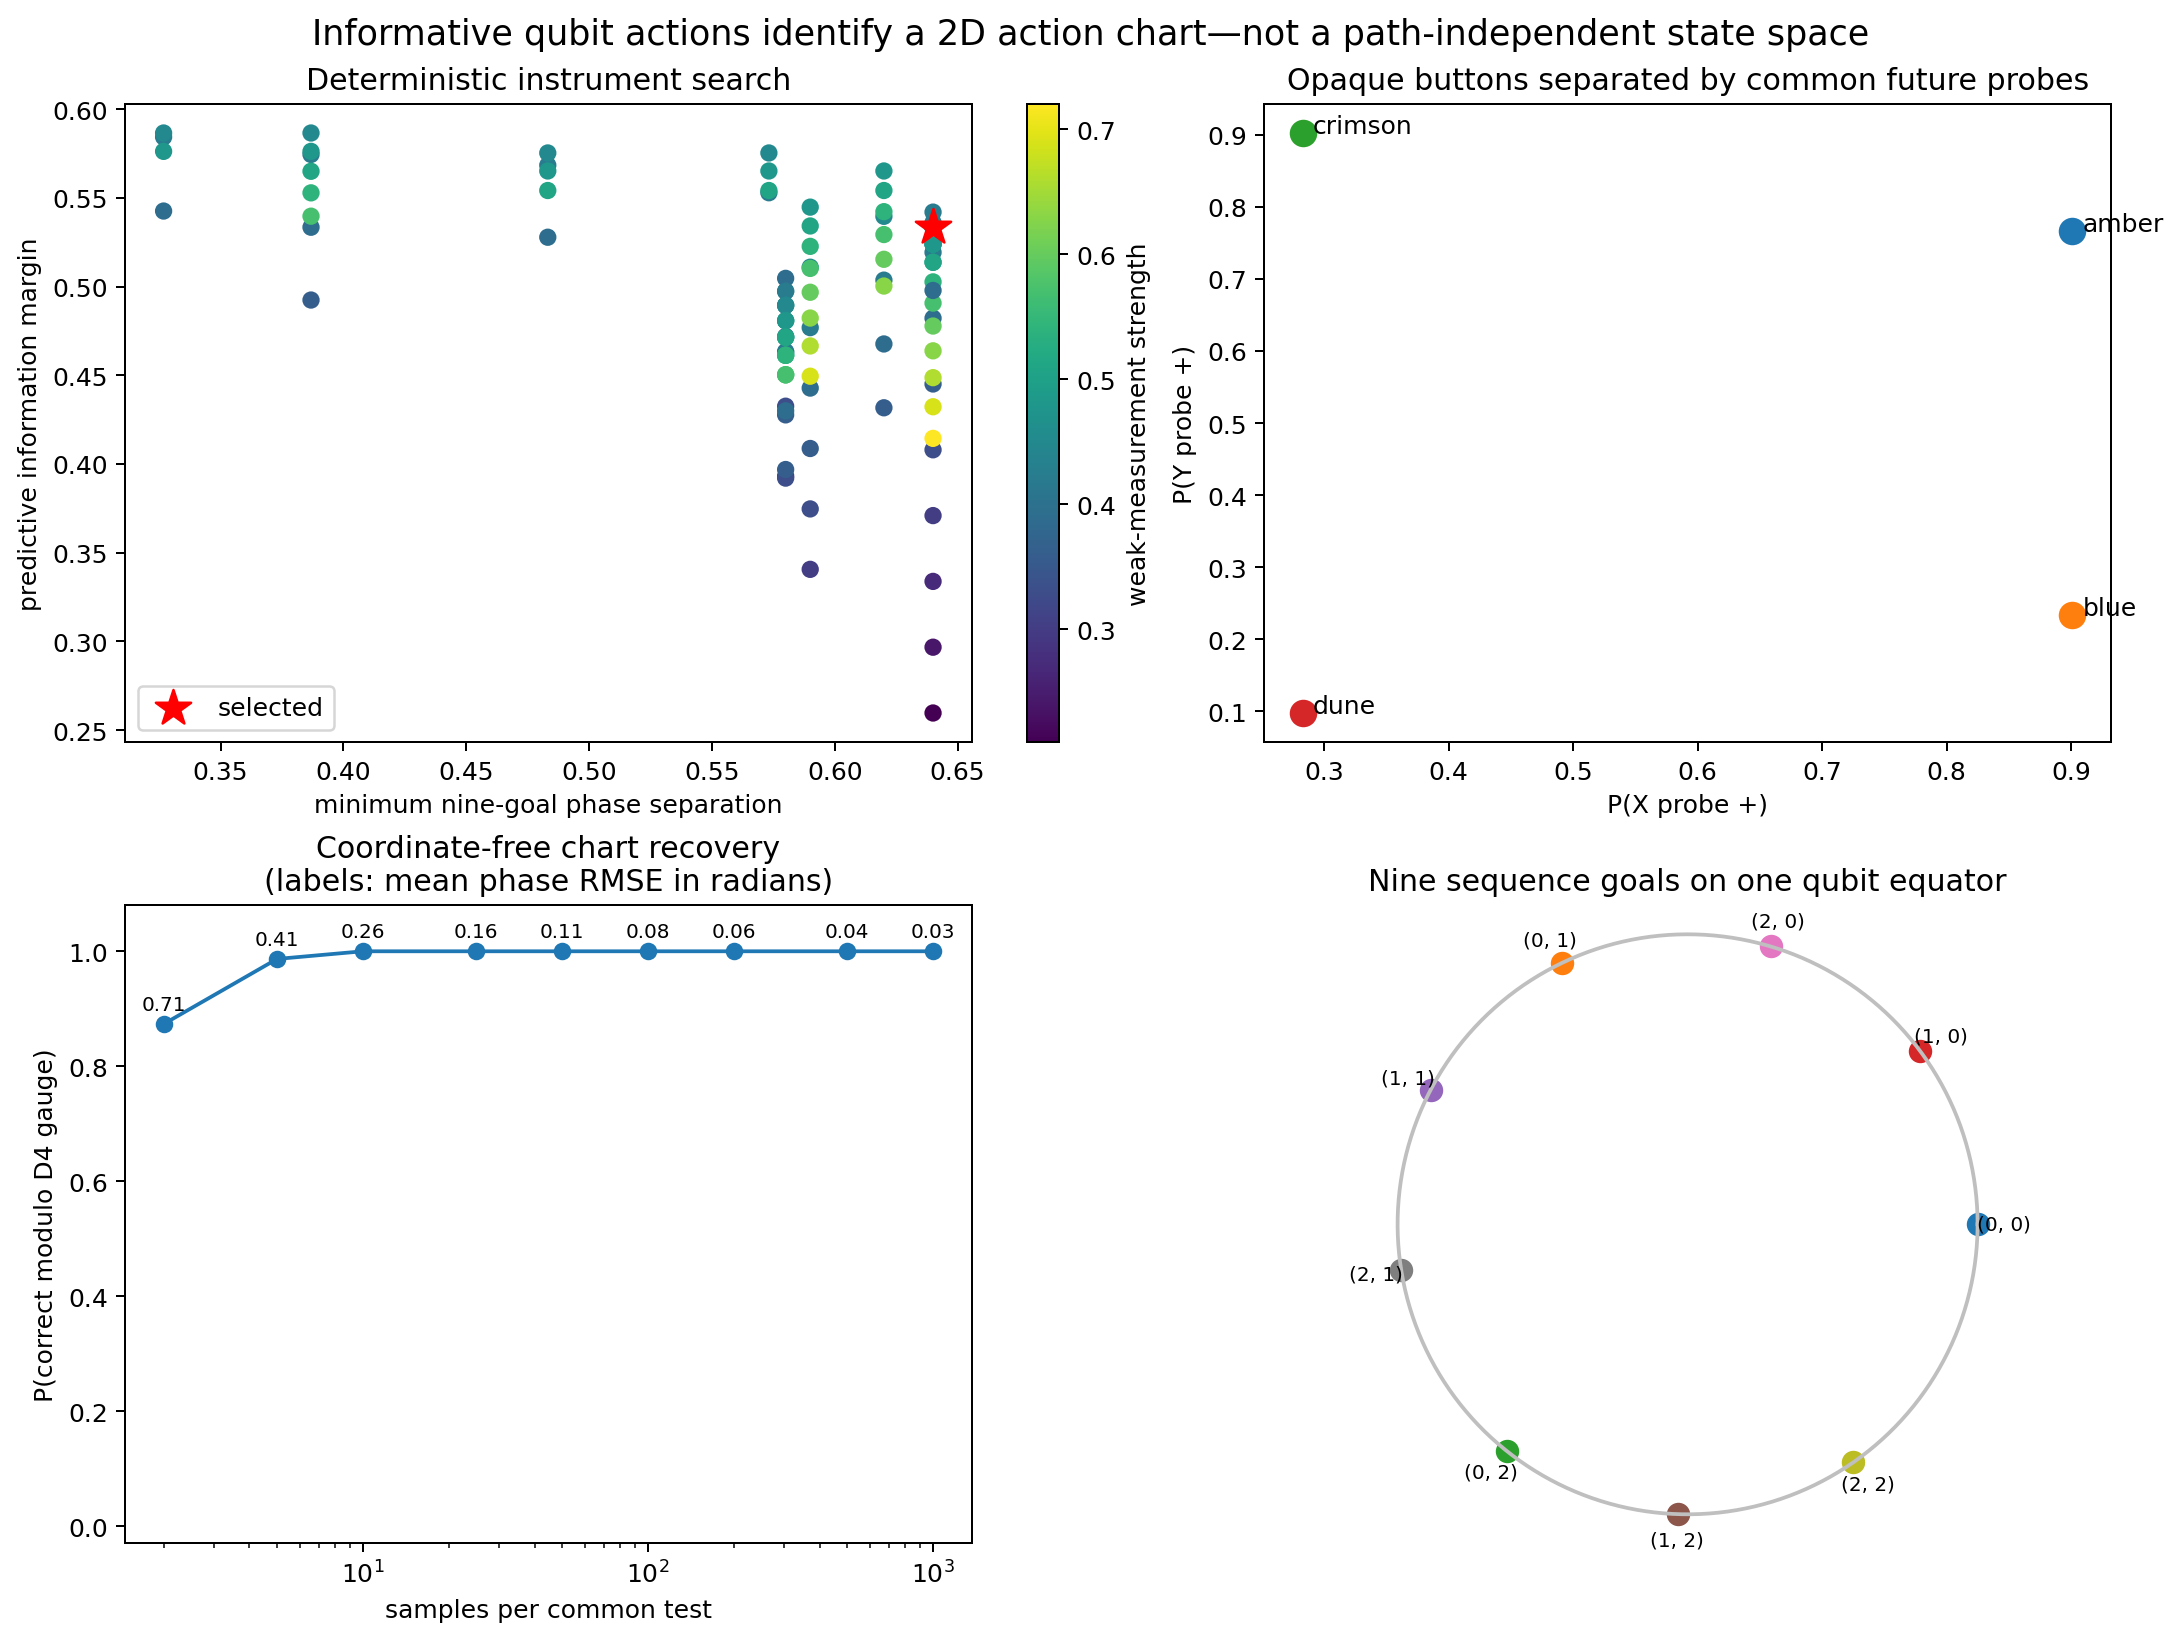
\includegraphics[width=.97\linewidth]{informative_qubit_summary.png}
\caption{Qubit predictive-semantics experiment. The action's immediate outcome
contains cosine information, while future \(X\) and \(Y\) probes provide an
invertible phase chart. Finite-sample reconstruction converges rapidly after
quotienting by chart symmetries.}
\label{fig:qubit-summary}
\end{figure}

\subsection{Decisive controls: meaning need not be immediate}

At \(200\) trials per setting, the informative nonunitary construction
recovered the action chart in every replicate. A random-unitary control with a
fair, state-independent current coin also achieved \(100\%\) action recovery
when future probes were allowed: the action changed the future state even
though its current outcome carried zero information. A null control achieved
\(0\%\). This establishes the logical distinction:
\[
I(S;O_t\mid A_t)=0
\quad\not\!\Longrightarrow\quad
\text{action has no predictive meaning}.
\]
The correct test is separation of shifted Hankel blocks, not immediate mutual
information alone.

\subsection{Why the nonunitary qubit does not furnish an exact plane}
\label{sec:qubit-failure}

An external finite history language can associate words in the two rotations
with nine declared displacement classes and thereby reproduce a \(3\times3\)
Manhattan chart. That statement is exact for the \emph{language automaton}.
It is not exact for the physical nonselective qubit dynamics.

Let \(D_X\) be the unsharp-measurement dephasing map on Bloch vectors,
\[
D_X(x,y,z)=(x,\eta y,\eta z),
\]
and let \(R_Z(\theta)\) be the rotation. The actual outcome-forgotten action is
\[
\Phi_\theta=D_X\circ R_Z(\theta).
\]
For two phases,
\[
\Phi_\alpha\Phi_\beta=D_XR_Z(\alpha)D_XR_Z(\beta),
\qquad
\Phi_\beta\Phi_\alpha=D_XR_Z(\beta)D_XR_Z(\alpha).
\]
Unless \(\eta=1\), or angles fall in special degenerate cases, \(D_X\) does
not commute with \(R_Z\), and these expressions differ. Thus words with the
same formal displacement can have different future statistics.

\begin{proposition}[Compositionality obstruction for the qubit family]
For \(0<s<1\) and generic nonzero \(\alpha,\beta\), the nonselective maps
\(\Phi_\alpha,\Phi_\beta\) do not commute. Consequently no quotient that
identifies all words solely by the net counts of \(\alpha\) and \(\beta\) is
an exact predictive-state quotient.
\end{proposition}
\begin{proof}
In the equatorial plane,
\[
D_XR_Z(\theta)=
\begin{pmatrix}
\cos\theta&-\sin\theta\\
\eta\sin\theta&\eta\cos\theta
\end{pmatrix}.
\]
Direct multiplication shows that the commutator has entries proportional to
\((1-\eta)\sin\alpha\sin\beta\) and related generic terms. It is therefore
nonzero outside the stated degeneracies. Two word histories related only by
exchange of \(\alpha\) and \(\beta\) then produce different states, separated
by some informationally complete future probe.
\end{proof}

The exhaustive check through word length four makes the size of the failure
explicit: among \(41\) formal displacement classes, \(33\) were represented by
multiple words, none of those \(33\) was path independent at tolerance
\(10^{-10}\), and the largest within-class predictive probe-vector difference
was \(0.128490\). The remaining eight classes were singletons and hence did
not test path independence.

\begin{figure}[H]
\centering
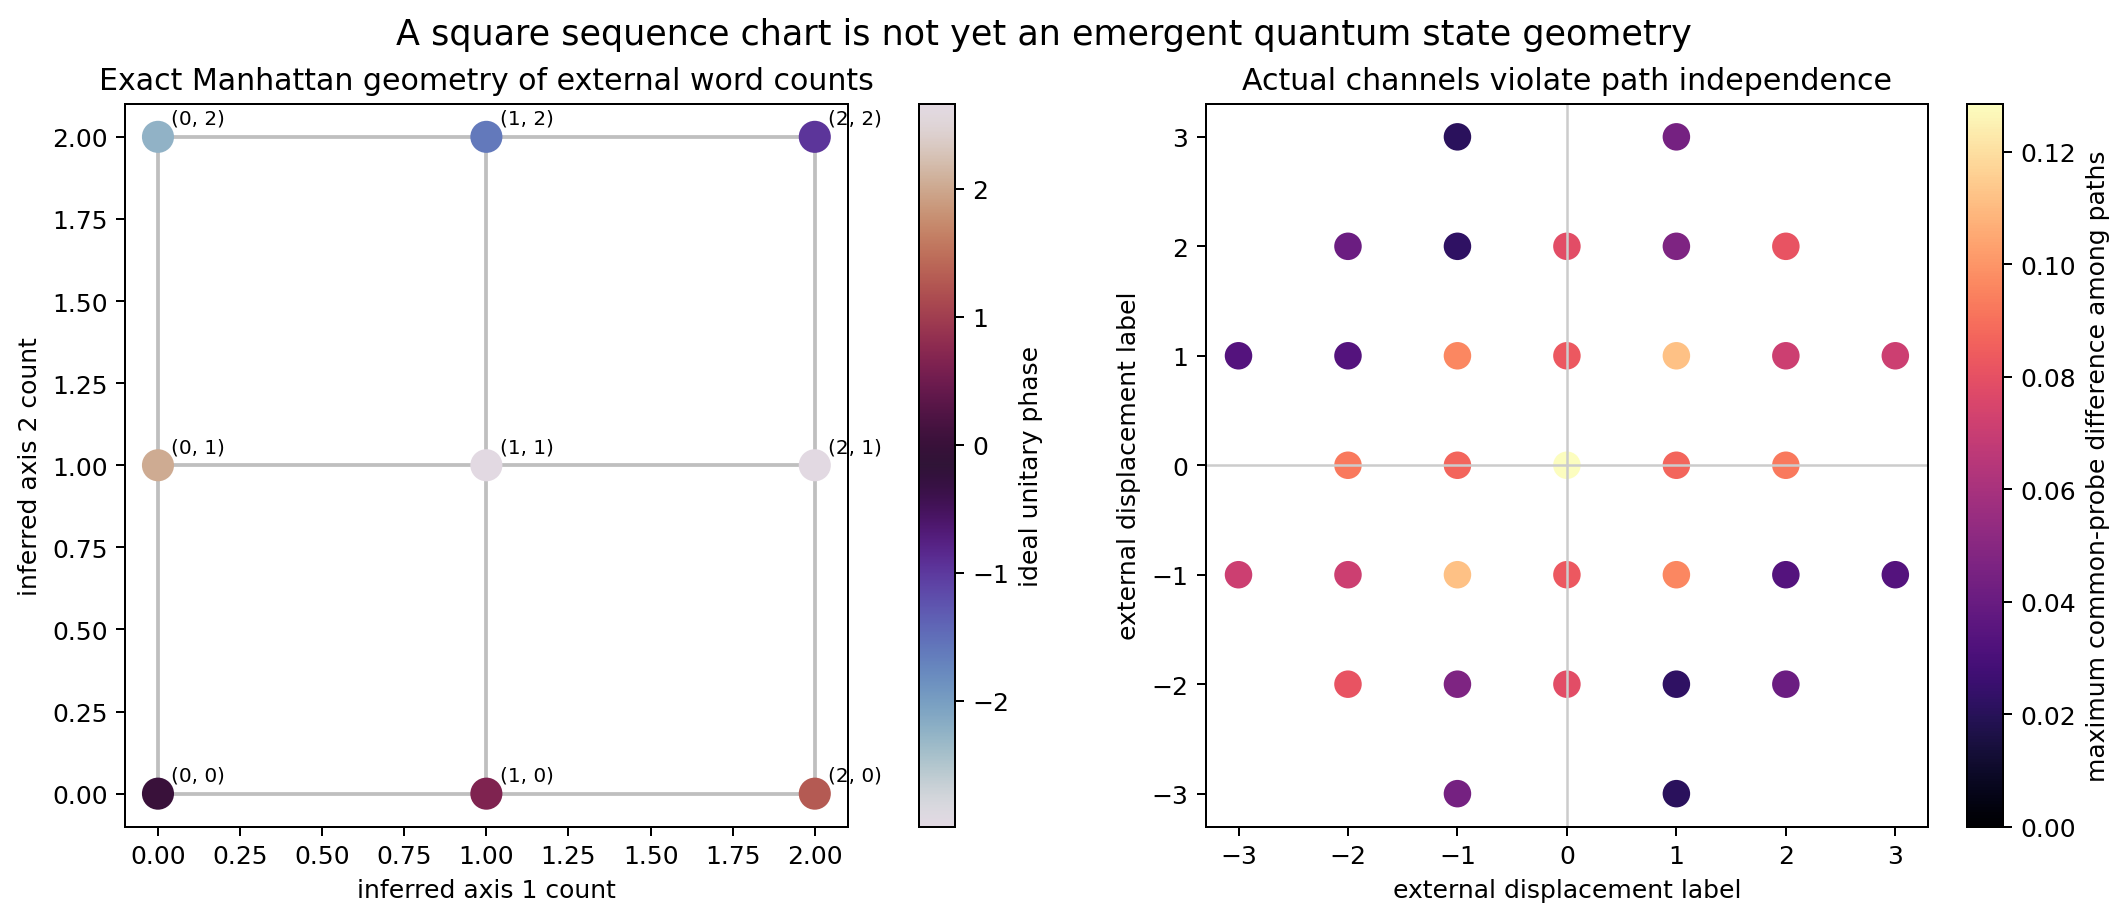
\includegraphics[width=.94\linewidth]{predictive_compositionality.png}
\caption{Honest compositionality audit. Words that an external displacement
automaton identifies need not be predictively equivalent under the physical
nonunitary qubit channels. The learned object is an action chart, not an exact
two-dimensional predictive-state space.}
\label{fig:qubit-composition}
\end{figure}

The limit \(s\to0\) sends \(\eta\to1\) and restores unitary composition, but
also eliminates immediate measurement information. Future probes can still
identify actions, yet an integrated instrument that both reports and composes
exactly remains unavailable in this family. This is a concrete manifestation
of \cref{thm:noinfo}.

\section{Qutrit case study: a learned Hesse-SIC action topology}
\label{sec:qutrit}

\subsection{The nine Hesse states}

Let \(\omega=e^{2\pi i/3}\), and define qutrit Weyl operators
\[
X|j\rangle=|j+1\bmod3\rangle,\qquad
Z|j\rangle=\omega^j|j\rangle.
\]
Starting from
\[
|\psi_{00}\rangle=\frac1{\sqrt2}(0,1,-1)^T,
\]
form the Weyl orbit
\[
|\psi_{mn}\rangle=X^mZ^n|\psi_{00}\rangle,\qquad
(m,n)\in\Z_3^2,
\]
and \(\Pi_{mn}=|\psi_{mn}\rangle\langle\psi_{mn}|\). These are the nine
Hesse symmetric informationally complete states. They satisfy
\begin{equation}
\label{eq:sic}
\frac13\sum_{m,n}\Pi_{mn}=I,\qquad
\Tr(\Pi_s\Pi_t)=
\begin{cases}
1,&s=t,\\
\frac14,&s\ne t.
\end{cases}
\end{equation}
The first identity says that \(\{\Pi_s/3\}\) is a POVM; the second says all
distinct pairs have equal quantum overlap.

The action set is
\[
\cA=\{I,X,X^\dagger,Z,Z^\dagger\}.
\]
Conjugation permutes the SIC orbit. We write
\[
U_a\Pi_sU_a^\dagger=\Pi_{T_a(s)}.
\]
Although \(XZ=\omega^{-1}ZX\) as operators, their conjugation actions commute:
the global phase disappears. Therefore the learned transformations can close
as translations of \(\Z_3^2\).

\subsection{One instrument that both moves and reports}

Define the integrated instrument
\begin{equation}
\label{eq:hesse-instrument}
K_o^{(a)}=\frac1{\sqrt3}\Pi_oU_a,\qquad
\cE_o^a(\rho)=K_o^{(a)}\rho K_o^{(a)\dagger}.
\end{equation}
Completeness is immediate:
\[
\sum_oK_o^{(a)\dagger}K_o^{(a)}
=U_a^\dagger\left(\frac13\sum_o\Pi_o\right)U_a=I.
\]
For an input SIC state \(\rho_s=\Pi_s\),
\begin{align}
p_a(o\mid s)
&=\Tr[K_o^{(a)}\Pi_sK_o^{(a)\dagger}]\\
&=\frac13\Tr[\Pi_oU_a\Pi_sU_a^\dagger]\\
&=\begin{cases}
\frac13,&o=T_a(s),\\[2pt]
\frac1{12},&o\ne T_a(s).
\end{cases}
\label{eq:hesse-likelihood}
\end{align}
Moreover, whenever the outcome has nonzero probability,
\[
\frac{K_o^{(a)}\Pi_sK_o^{(a)\dagger}}{p_a(o\mid s)}=\Pi_o.
\]
Thus the action first translates the likelihood peak, while the emitted token
also becomes the exact next predictive state. The last outcome is a sufficient
statistic for all future behavior. This measure-and-prepare structure makes
the model exactly solvable.

Under a uniform prior on the nine source states, the immediate mutual
information is
\begin{align}
I(S;O\mid a)
&=\log_2 9-
H\left(\frac13,\underbrace{\frac1{12},\ldots,\frac1{12}}_{8}\right)\\
&=0.251629\ \text{bits}.
\label{eq:hesse-mi}
\end{align}
The information is modest but strictly positive.

\subsection{Learning topology from opaque tokens}

For the learning experiment, both source-state identifiers and action
identifiers were independently shuffled. The learner was not supplied the
coordinate labels \((m,n)\), the words \(X,Z\), or the direction names.
With \(2{,}000\) samples for each source--action pair, empirical likelihood
tables estimated the peak map
\[
\widehat T_a(s)=\arg\max_o\widehat p_a(o\mid s).
\]
All \(45=9\times5\) peak images were recovered correctly. Mean absolute
probability error per action lay between \(0.00505\) and \(0.00579\).

Purely algebraic diagnostics then found:
\begin{itemize}
\item one learned permutation was the identity and had order one;
\item the other four had order three;
\item all learned permutations commuted;
\item they generated a group of order nine;
\item the orbit of any token contained all nine tokens.
\end{itemize}
These are observable signatures of a \(\Z_3\times\Z_3\) regular action, up to
permutation and lattice-automorphism gauge. Hence the words horizontal and
vertical are interpretations assigned \emph{after} recovery, not labels used
to train the estimator.

\begin{figure}[H]
\centering
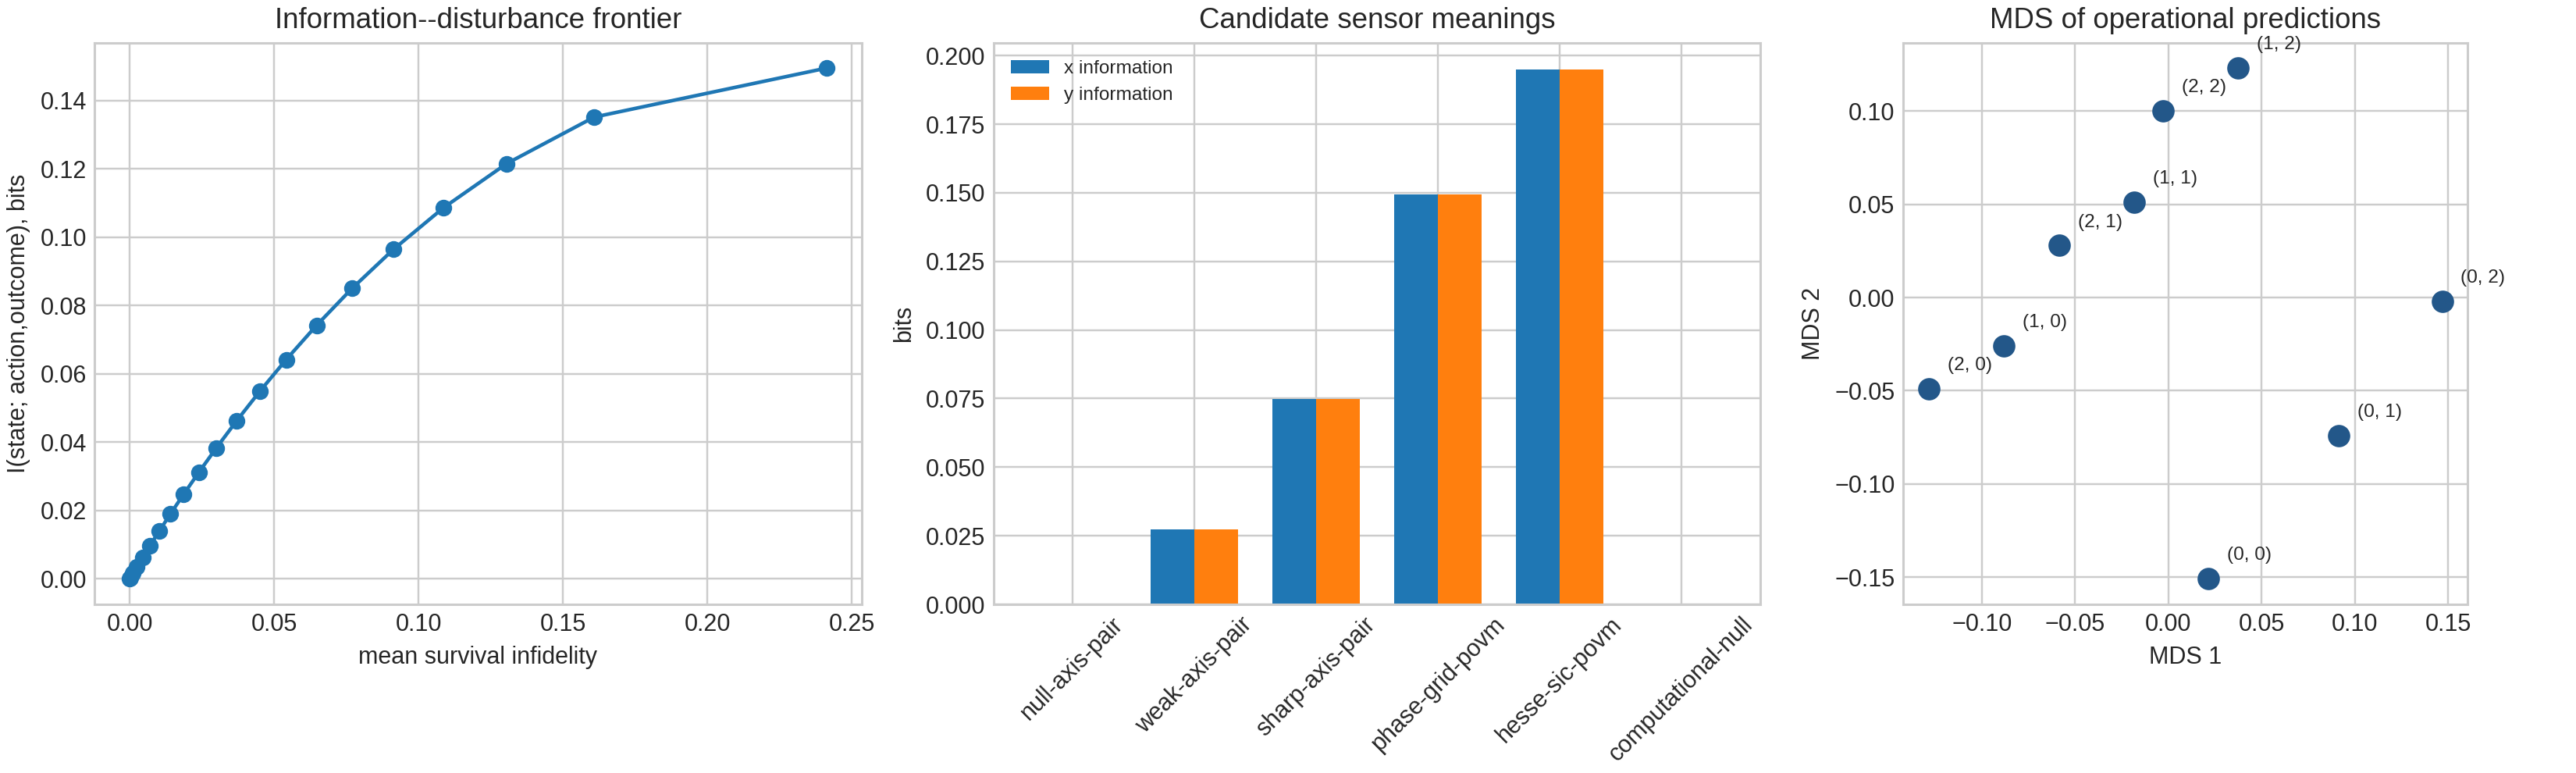
\includegraphics[width=.97\linewidth]{candidate_search_and_geometry.png}
\caption{Qutrit candidate and geometry diagnostics. The Hesse-SIC orbit makes
every off-diagonal quantum overlap equal, while the action permutations
recover a two-generator finite topology. The toroidal word distance has
substantial planar MDS distortion and must not be confused with an exact
Euclidean metric.}
\label{fig:qutrit-candidate}
\end{figure}

The Cayley graph with generators \(X^{\pm1},Z^{\pm1}\) is a \(3\times3\)
torus. Its graph distance \(d_T\) has shells \(0,1,2\) with multiplicities
\(1,4,4\). This is unambiguously two-generator and translation covariant.
However, two-dimensional metric MDS has stress \(0.383\). A torus can be
topologically two-dimensional without its all-pairs shortest-path metric
being a Euclidean planar distance. This is the first warning that recovered
topology is weaker than recovered geometry.

\section{The exact integrated Bellman obstruction}
\label{sec:no-go}

\subsection{Goal protocol and exact solution}

Fix a goal token \(g\). Each integrated action costs one. The episode stops
when the reported outcome is \(g\); otherwise the next predictive state is the
reported SIC state. The undiscounted Bellman equation is
\begin{equation}
\label{eq:integrated-bellman}
V_g(s)=\min_a\left[
1+\sum_{o\ne g}p_a(o\mid s)V_g(o)
\right].
\end{equation}
Translation and dihedral symmetries imply that the value depends only on the
toroidal shell. Write \(v_0,v_1,v_2\) for self, edge, and diagonal,
respectively.

At the goal, the identity action centers the likelihood at \(g\). Its success
probability is \(1/3\); the four edge and four diagonal failures each have
probability \(1/12\). Hence
\begin{equation}
v_0=1+\frac13v_1+\frac13v_2.
\label{eq:v0}
\end{equation}
From an edge state, one translating action maps the premeasurement peak to
\(g\), producing exactly the same report kernel as identity at the goal.
Because both actions cost one and every failure branch is determined solely by
the outcome,
\begin{equation}
v_1=1+\frac13v_1+\frac13v_2=v_0.
\label{eq:v1}
\end{equation}
From a diagonal state, an optimal cardinal move centers the report at a state
adjacent to \(g\). Among nonsuccess outcomes, the center and three further
edge tokens contribute total coefficient \(1/3+3/12=7/12\), while four
diagonal tokens contribute \(4/12=1/3\). Therefore
\begin{equation}
v_2=1+\frac7{12}v_1+\frac13v_2.
\label{eq:v2}
\end{equation}
Solving \cref{eq:v0,eq:v1,eq:v2} gives
\begin{equation}
\boxed{v_0=4,\qquad v_1=4,\qquad v_2=5.}
\label{eq:exact-values}
\end{equation}
Direct enumeration of the five Bellman actions verifies the assumed
minimizers and the minimal nonnegative solution.

\begin{proposition}[Exact self--edge no-go for the report-again Hesse protocol]
The goal-normalized cost \(C(s,g)=V_g(s)-V_g(g)\) is zero for every state
adjacent to \(g\). It therefore violates identity of indiscernibles and cannot
be a metric, regardless of embedding algorithm.
\end{proposition}
\begin{proof}
Equation \cref{eq:exact-values} gives \(V_g(s)=V_g(g)=4\) for an edge state.
Thus \(C(s,g)=0\) although \(s\ne g\).
\end{proof}

\paragraph{Terminal-semantics correction.}
This proposition concerns the event goal ``make the instrument report \(g\)
again,'' so another intervention is charged even when the present predictive
state is already \(g\). It is not a no-go for state-hitting hodology. For the
place-like goal ``the current predictive state is \(g\),'' the Bellman boundary
is instead \(V_g(g)=0\). Keeping the same transition kernel, the edge and
diagonal equations give \(V_{\rm edge}=4\) and
\(V_{\rm diagonal}=5\), hence the strict metric shells \((0,4,5)\). The
covariant-memory successor develops this corrected semantics and adds
full-rank retained-memory branches. Thus the calculation above remains exact,
but its scope is an event/report cost rather than distance from the present
state to a place.

\begin{figure}[H]
\centering
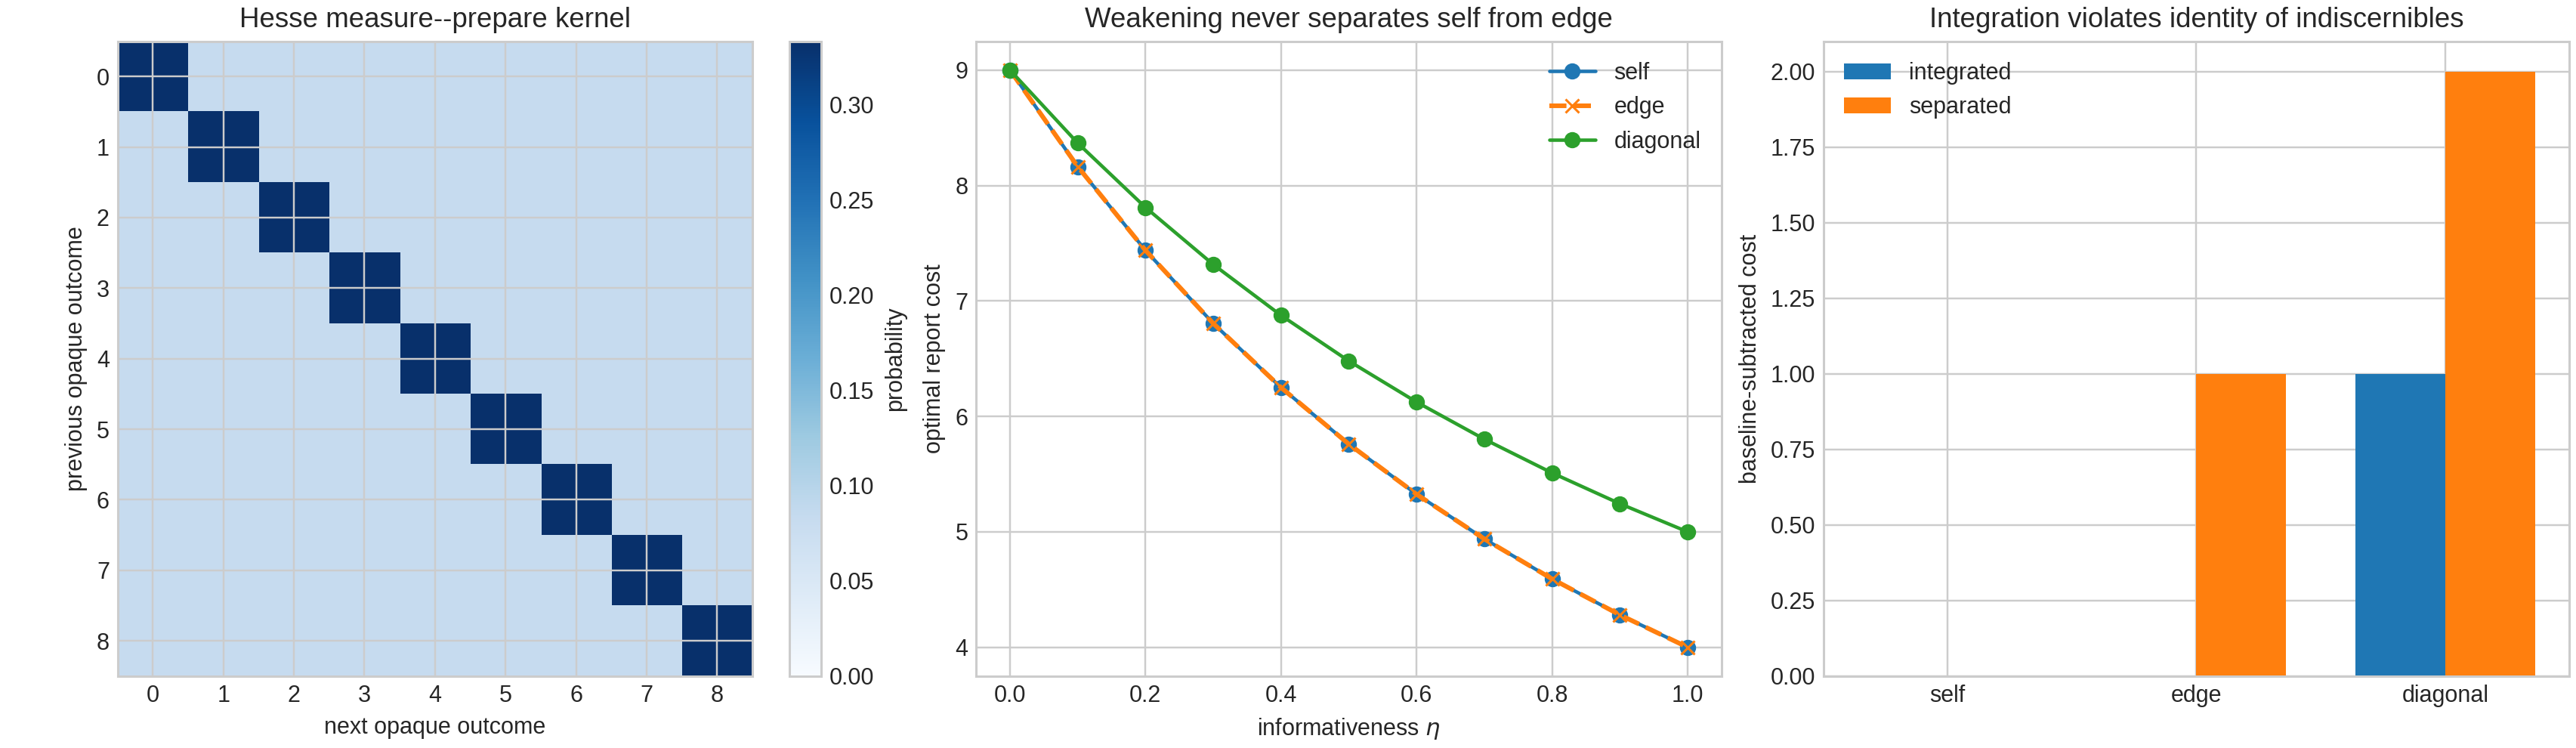
\includegraphics[width=.98\linewidth]{integrated_action_no_go.png}
\caption{The central negative result. The integrated Hesse-SIC instrument
learns a clean opaque action topology, yet exact Bellman analysis yields equal
self and edge costs. Weakening the report preserves this equality. The
separated move/report benchmark recovers toroidal distance only by giving up
integration.}
\label{fig:integrated-no-go}
\end{figure}

\subsection{Why weakening the measurement does not fix it}

Mix the exact likelihood with uniform noise:
\begin{equation}
\label{eq:weak-family}
p_a^\eta(o\mid s)=
\eta p_a(o\mid s)+\frac{1-\eta}{9},
\qquad 0\le\eta\le1.
\end{equation}
This has a physical measure-and-prepare realization with effects
\[
F_o^\eta=\frac{\eta}{3}\Pi_o+\frac{1-\eta}{9}I
\]
and posterior preparation \(\Pi_o\). The same branch-state reset remains.

\begin{table}[H]
\centering
\caption{Exact Bellman shell values for the weak integrated family. Numerical
rounding is shown to three decimals. Self and edge remain exactly equal
throughout the family.}
\label{tab:weak-values}
\begin{tabular}{cccc}
\toprule
\(\eta\) & self \(v_0\) & edge \(v_1\) & diagonal \(v_2\)\\
\midrule
0.0 & 9.000 & 9.000 & 9.000\\
0.2 & 7.438 & 7.438 & 7.810\\
0.4 & 6.250 & 6.250 & 6.875\\
0.6 & 5.325 & 5.325 & 6.124\\
0.8 & 4.592 & 4.592 & 5.510\\
1.0 & 4.000 & 4.000 & 5.000\\
\bottomrule
\end{tabular}
\end{table}

The equality is structural. For an edge state, an aligning move followed by
the report has the same outcome kernel as identity followed by the report at
the goal. Since (i) both cost one and (ii) every outcome prepares the same
\(\Pi_o\) independent of the source, their Bellman action values coincide for
every \(\eta\). Making the measurement weak changes the common value but not
the degeneracy. The obstruction is therefore not simply too much
measurement; it is the combination of equal move/report cost and complete
outcome-only reset.

\subsection{Separated motion and report: an exact benchmark, not a solution}

As a diagnostic control, allow noiseless unitary translations as actions and
a separate Hesse-SIC report action. The agent can first move to \(g\), then
report. At \(g\), one report attempt costs one and succeeds with probability
\(1/3\). A failed report prepares one of four edge states or four diagonal
states, each with probability \(1/12\); the mean cost of returning to \(g\) is
\[
4\left(\frac1{12}\right)(1)+
4\left(\frac1{12}\right)(2)=1.
\]
If \(v\) is the value at the goal,
\[
v=1+1+\frac23v,
\qquad\text{so}\qquad v=6.
\]
Starting at \(s\), first pay the exact toroidal word distance. Thus
\begin{equation}
\boxed{V_g(s)=6+d_T(s,g).}
\label{eq:separated}
\end{equation}
Subtracting the self cost gives exactly \(d_T\). This confirms that the goal
protocol and Bellman solver can recover a nondegenerate graph geometry. It
does not demonstrate an integrated informative translation: the unitary move
emits no spatial information, and measurement is delegated to a distinct
action.

\section{Computational evidence and controls}

The analytic statements above were accompanied by deterministic finite-sample
experiments.  This section explains what the numerical diagnostics add beyond
the proofs.

\subsection{Why these metrics were chosen}

Kernel mean absolute error tests whether the learned controlled probability
law is quantitatively calibrated.  Permutation recovery tests the discrete
action algebra while respecting token gauge.  Held-out negative log
likelihood asks whether a learned predictive state generalizes beyond the
strings used to identify it.  Bellman residual checks that an alleged distance
is actually induced by optimal behavior.  Identity of indiscernibles is tested
before MDS, because no embedding can rescue two distinct predictive states at
zero cost.  Finally, path closure asks whether the same inferred displacement
has the same future law along different routes.  These tests address different
possible false positives and none can substitute for the others.

For the qubit, 11,799 deterministic parameter triples were searched.  With
300 replications, recovery of the opaque two-axis chart was 0.873, 0.987, and
1.000 at two, five, and ten samples per common test.  Predictive tomography
from 300 samples of each Pauli probe had mean trace-distance error 0.035.  Yet
zero of 33 repeated-path displacement classes closed predictively, with worst
common-probe discrepancy 0.12849.

For the qutrit, 2,000 observations for every source-token/action pair recovered
all 45 images of the five hidden permutations.  Per-entry controlled-kernel
error ranged from 0.00505 to 0.00579.  The production bundle also contains
20,000 training and 8,000 held-out five-step sequences and 34,000 navigation
episodes.  These data verify learnability and prediction; the exact Bellman
plateau remains an analytic failure independent of sampling noise.

\begin{figure}[H]
\centering
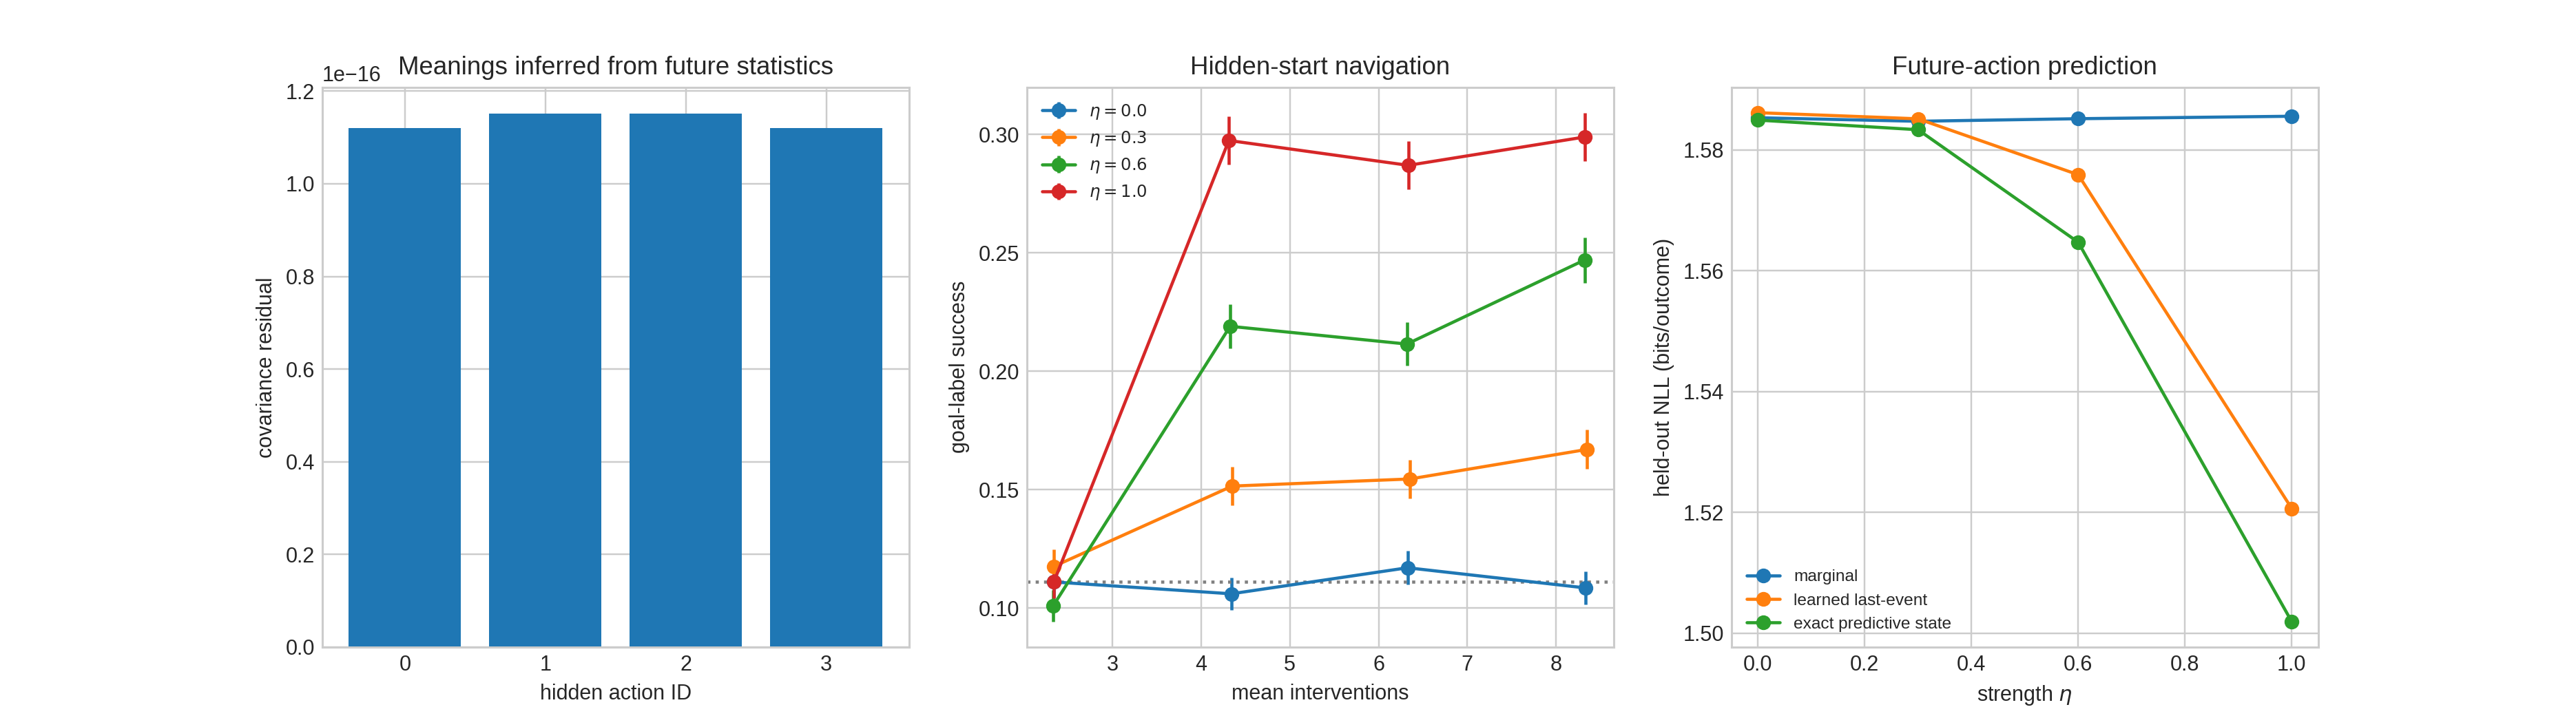
\includegraphics[width=.98\linewidth]{action_meanings_navigation_prediction.png}
\caption{Operational qutrit diagnostics.  Opaque actions are inferred from
future statistics, informative strength improves hidden-start behavior and
held-out prediction, and all evaluation occurs without exposing coordinates
to the learner.  These positive diagnostics coexist with the exact metric
failure in \cref{fig:integrated-no-go}.}
\label{fig:qutrit-learning}
\end{figure}

\subsection{Matched skeptical controls}

Four controls locate the source of apparent geometry.
\begin{enumerate}
\item A random-unitary catalog has zero immediate mutual information but can
still be distinguished by future probes.  Thus immediate outcomes are not
necessary for operational action semantics.
\item A null quantum channel has rank-zero response variation and supports no
quantum action chart.
\item A nine-state external automaton can retain a Manhattan label grid while
the quantum state is constant.  This shows why word counts are not evidence of
predictive quantum space.
\item Independent permutations of actions and outcomes leave all invariant
claims unchanged.  Coordinate names and compass directions are gauges, not
observables.
\end{enumerate}
The controls jointly reject both extremes: neither ``the outcome was
uninformative, so the action has no meaning'' nor ``the word graph looked
spatial, so space emerged'' is valid.

\section{What has and has not been established}

\begin{table}[H]
\centering
\caption{The constructions pass different parts of the operational contract.
An entry ``future'' means that semantics is identifiable by later common tests
although the movement outcome itself is null.}
\begin{tabularx}{\linewidth}{lXXXX}
\toprule
Model & Information & Learned structure & Bellman result & Decisive limitation\\
\midrule
Pauli qubit square & future & exact four-place action semantics & Euclidean
square & movement outcome uninformative\\
Nonunitary qubit & immediate + future & robust two-axis chart & external
Manhattan words & 0/33 repeated paths close\\
Integrated Hesse qutrit & 0.251629 bits & exact opaque $\Z_3^2$ topology &
self=edge=4, diagonal=5 & pseudometric\\
Separated Hesse qutrit & report only & exact torus translations &
$6+d_T$ & movement outcome uninformative\\
Null quantum DFA & none & external labels only & arbitrary word graph & no
quantum predictive geometry\\
\bottomrule
\end{tabularx}
\end{table}

The central positive result is that the meanings of quantum actions can be
learned relationally from controlled observations in Hilbert dimension two or
three.  The Hesse construction further proves that informative integrated
actions can reveal an exact two-generator topology.  The central negative
result is equally precise: in the minimal symmetric measure-and-prepare
family, information-producing backaction erases the strict Bellman separation
between a goal and its neighbors.  Therefore topology, observability, and
low-dimensional hodological metric are logically independent requirements.

The no-information theorem is not a universal ban on informative geometric
motion.  Its assumptions include branchwise pure-state translation and
universal nondisturbance on a connected nonorthogonality graph.  Mixed-state
memory, non-rank-one effects, outcome-conditioned displacement, approximate
closure, or an enlarged predictive fiber can evade those assumptions.  Such
evasions must be charged in the predictive state rather than hidden in a
coordinate counter.

\section{Most promising next direction}

The next experiment should search outcome-conditioned, group-covariant qutrit
channels with retained quantum memory.  Rather than choosing a geometric
target after simulation, optimize one family jointly against the finite
certificate:
\begin{enumerate}
\item positive immediate mutual information, bounded away from zero;
\item predictive separation and held-out sequence likelihood;
\item identifiable inverse action pairs and low algebra residual;
\item path closure for commuting squares and longer held-out words;
\item a proper Bellman solution with strict
$V_{\rm self}<V_{\rm edge}<V_{\rm diagonal}$;
\item a symmetric metric with a positive-semidefinite rank-two Schoenberg
Gram matrix, or a controlled approximation whose error is reported;
\item null, cloned-action, random-unitary, episode-rescrambled, and external-DFA
controls.
\end{enumerate}

A practical parametrization is to tie Kraus branches covariantly,
\(\cE^{a}_{o}=\cU_a\circ\mathcal F_{T_a^{-1}o}\), while allowing each fiducial map
\(\mathcal F_o\) to have rank larger than one. Rank-one measure-and-prepare maps
erase too much memory; higher-rank branches may report partial location while
preserving the phase information required for composition.  A differentiable
inner Bellman solver can evaluate shell margins, while an outer constrained
optimizer enforces complete positivity and trace preservation.  Candidates
must then be relearned from sampled opaque histories by a spectral predictive
state model, so success cannot depend on access to their matrices.

This program also offers a disciplined route toward a fiber bundle.  The
translation quotient would form the base; residual predictive distinctions
left after fixing place would form the fiber.  Commutator loops of learned
action operators could then measure operational holonomy.  Curvature and
spacetime analogies should be deferred until a flat, informative baseline
passes every condition above.

\section{Reproduction and data provenance}

From the directory containing this paper, run
\begin{verbatim}
cd qubit
python -m unittest discover -s tests -v
MPLBACKEND=Agg python run_qubit_experiment.py
cd ../qutrit
python -m unittest -v test_informative_qutrit.py
MPLBACKEND=Agg python informative_qutrit.py --episodes 2000 --seed 20260812
\end{verbatim}
The qubit and qutrit strands contain seven and nine focused tests,
respectively.  Saved CSV and JSON files include exact kernels, parameter-search
rankings, finite-sample recovery, word-equivalence audits, information--
disturbance sweeps, Bellman matrices, held-out prediction, navigation, controls,
and complete manifests.  Hidden permutations and coordinates are used only
for frozen evaluation, never as learner inputs.

\section{Conclusion}

The user's criticism of dead reckoning changes the standard of evidence in a
productive way.  A spatial action is not defined by a matrix name, nor by an
external counter updated when a button is pressed.  Its meaning is the
relational transformation it induces on the probabilities of future
experience.

Under that standard, a qubit already supports learnable two-direction action
semantics, and a qutrit supports an exactly learnable $\Z_3^2$ translation
topology with genuinely informative outcomes.  But the strongest integrated
candidate is not a hodological metric: self and neighbor have equal optimal
report cost.  No current model in this study simultaneously achieves
informative integrated action, predictive path closure, and a nondegenerate
exact two-dimensional metric.  This honest obstruction supplies the right
objective for the next generation of quantum environments.

\begin{thebibliography}{99}
\bibitem{Kraus1983} K.~Kraus, \emph{States, Effects, and Operations}
(Springer, 1983).
\bibitem{NielsenChuang2010} M.~A. Nielsen and I.~L. Chuang,
\emph{Quantum Computation and Quantum Information}, anniversary ed.
(Cambridge University Press, 2010).
\bibitem{Watrous2018} J.~Watrous, \emph{The Theory of Quantum Information}
(Cambridge University Press, 2018).
\bibitem{Littman2001} M.~L. Littman, R.~S. Sutton, and S.~Singh,
``Predictive representations of state,'' \emph{NeurIPS 14} (2001).
\bibitem{NielsenGST2020} E.~Nielsen et al., ``Gate Set Tomography,''
arXiv:2009.07301 (2020).
\bibitem{DiMatteo2020} O.~Di Matteo et al., ``Operational, gauge-free quantum
tomography,'' arXiv:2007.01470 (2020).
\bibitem{Puterman1994} M.~L. Puterman, \emph{Markov Decision Processes}
(Wiley, 1994).
\bibitem{SuttonBarto2018} R.~S. Sutton and A.~G. Barto,
\emph{Reinforcement Learning: An Introduction}, 2nd ed. (MIT Press, 2018).
\bibitem{Schoenberg1935} I.~J. Schoenberg, ``Remarks to Maurice Fr\'echet's
article,'' \emph{Annals of Mathematics} 36, 724--732 (1935).
\end{thebibliography}

\end{document}
